\section{Jaké jsou základní měřitelné parametry kvality služeb v multimediálních sítích? Popište, jakým způsobem se zajišťuje kvalita služeb prostřednictvím integrovaných (Intserv) a diferencovaných (Diffserv) služeb, diskutujte hlavní rozdíly. K čemu slouží QoE?}

Kvalita služeb -- Vhodně definované a kontrolované chování systému v souladu s kvantitativně měřitelnými parametry

Základné merateľné parametre: 
\begin{itemize}
    \item Propustnost/šířka pásma (Throughput/Bandwidth) [bit/s] -- Maximální dlouhodobá rychlost přenosu = maximální počet datových jednotek přenesených za jeden časový interval (paket/s)
    \item Zpoždění [ms] -- \textbf{Paketizační} (Časový interval na zpracování dat na koncové stanici) a \textbf{Propagační} (Časová interval na přenos dat na médiu)
    \item Kolísání zpoždění [ms] -- Maximální povolená časová odchylka doručení dat do cíle
    \item Ztrátovost/spolehlivost  [/\%] -- \textbf{Loss rate} (maximální počet ztrát v jeden časový interval) \textbf{Loss size} (maximální počet po sobě ztracených paketů)
    \item Bezpečnost
    \item Cena
    \item Stabilita (Pružnost)
\end{itemize}

\subsection{Intserv -- Integrované služby}
První model pro zajištění QoS, Rezervace pro každé spojení zvlášť, Tok dat definovaný jako proud souvisejících paketů, Poskytuje \textbf{garantovanou} službu i službu s \textbf{řízením zátěže}

Nevýhody: 
\begin{itemize}
    \item Velké nároky na směrovače -- Musí umět zpracovávat velké množství datových toků
    \item Orientace RSVP protokolu na přijímač -- Přijímač musí být iniciátorem rezervace zdrojů sítě
    \item Opakovaná rezervace síťových prostředků dodatečně zatěžuje síť
    \item Vhodné pro delší audio/video
\end{itemize}

\subsection{Diffserv -- Diferencované služby}
Neklade tak vysoké nároky na síť jako IntServ, Nevyžaduje sestavení cesty s definovanými parametry, Rozlišení probíhá v krajních směrovačích sítě nebo v koncových zařízeních, Jednotlivé pakety jsou označené podle typu služby v IP hlavičce, Řízení přístupu(admission control) je umístěno pouze v okrajových směrovačích sítě

Princip: V první fázi jsou mezi uživatelem a poskytovatelem připojení dohodnuty parametry pro přenos SLA (Service Level Agreement)

Nevýhody: 
\begin{itemize}
    \item Poskytování QoS datovým tokům na bázi per-hop nemůže zaručit garanci stále QoS na celé trase mezi koncovými uzly
    \item Statická konfigurace SLA mezi účastníkem a provozovatelem sítě
    \item Model DS je orientován pouze na vysílač
    \item Poskytování QoS pouze skupinám datových toků
\end{itemize}

\subsection{QoE -- Kvalita zážitků (Quality of Experience)}
Úzce souvisí s kvalitou služeb QoS, je zaměřena na subjektivní dojem uživatele a závisí jak na technických i
lidských faktorech

Možnost měřit : 
\begin{itemize}
    \item Subjektivně –- hodnocení z pohledu koncového uživatel
    \item Objektivně –- odhad QoE pomocí empirického modelu bez nutnosti zapojení uživatelů
\end{itemize}

\textbf{Faktory ovlivňující QoE}
\begin{itemize}
    \item Obsah (Závisí na tom, zda uživateli je či není obsah přívětivý)
    \item Uživatel (Výsledné hodnocení QoE je závislé na dojmech a očekáváních uživatele)
    \item Prostředí (Na výsledné hodnocení má vliv například okolní hluk, nedostatečné osvětlení apod.)
    \item Systém (Technické vybavení, které konkrétní služba využívá)
\end{itemize}

\newpage
\section{Popište výhody a nevýhody multicastového přenosu. Popište modely mulsticastu ASM, SSM, jejich rozdíly a funkci protokolu protokol IGMP.}

\subsection{Multicast}
Posílání kopie dat všem ve skupině, nutnost registrovat skupiny, skupina je reprezentovaná adresou IPv4 typu D – začínají 1110 (224.0.0.0 – 239.255.255.255), může být rozprostřena po celém Internetu, v jedné skupině může být i více vysílačů (Vysílače nemusí být členové skupiny), 
Výhody: 
\begin{itemize}
    \item Podpora směrovačů!!!
    \item IGMP protokol
    \item méně zatěžuje síť než vysílat UNICAST každé stanici
\end{itemize}

Nevýhody: 
\begin{itemize}
    \item Z principu jde o nespolehlivý protokol –- neexistuje spojení mezi vysílačem a přijímačem, router musí podporovat multicast, alokace adres, neefektivní řízení zdrojů, nutno ponechat složitější cestu v síti
\end{itemize}

2 typy 
\begin{itemize}
    \item Vysílání od jednoho uživatele k mnoha
    \item Vysílání od mnoha uživatelů k jednomu
\end{itemize}

\begin{figure} [h]
     \centering
     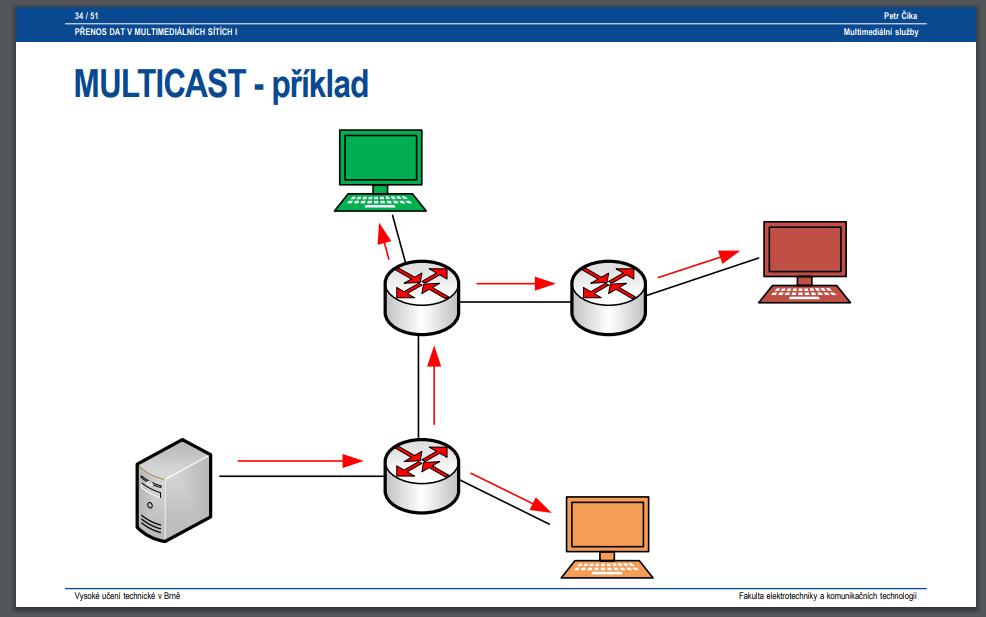
\includegraphics[width=0.85\textwidth]{images/multicast.PNG}
\end{figure}
\textbf{Využitie} -- IP televize, Vícebodové videokonference, Internetové rádio, Konfigurace skupin zařízení, Distribuce programového vybavení

Směrovací protokoly pro multicast -- Sparse Mode (SM), Dense Mode (DM), Link State (LS)

\textbf{Modely multicastu} -- ASM, SSM

\subsection{ASM (Any Source Multicast)}
Sdílený strom, 1 centrální směrovač – \textbf{Randezvous Point (RP)}, Může být více zdrojů – \textbf{nerozlišují se}

Komunikace: 
\begin{enumerate}
    \item paket IGMP
    \item Koncový směrovač zažádá o příjem RP
    \item RP začne vysílat
    \item Vlastní přenos
\end{enumerate}

\textbf{Využitie} -- Videokonference, on-line hry

\subsection{SSM (Source Specific Multicast)}
Zdrojový strom, vysílač je vždy kořen, pro každý zdroj je vytvořen strom nejkratších cest, Využívá rozsah adres 232.0.0.0 – 232.255.255.255, Může být více zdrojů – \textbf{rozlišují se}, Možnost používat jednu multicastovou adresu pro více zdrojů, Vhodné pro vysílání typu jeden k mnoha (broadcast)

Komunikace: 
\begin{enumerate}
    \item paket IGMP
    \item Je sestaven strom od vysílače až k přijímači.
    \item Vlastní přenos
\end{enumerate}

\textbf{Využitie} -- VoD (Video on Demand – video na vyžádání), e-learning

\subsection{IGMP (Internet Group Management Protocol)}
Využíván koncovými stanicemi k \textbf{připojení nebo odhlášení ze skupiny} -- Management skupin na síťové vrstvě\newline
Využívány koncovými stanicemi ke komunikaci s prvním směrovačem, \textbf{TTL vždy 1} -- vysílá vždy jen nejbližší stanici
Verze 1,2,3

\newpage
\section{Popište protokoly RTP a RTCP – k čemu protokoly slouží, jaké informace poskytují, kdy a proč se používají.}

\subsection{RTP -- Real-time transport protocol}
Poskytuje mechanizmy pro multimediální přenosy v reálném čase
\begin{enumerate}
    \item \textbf{Rekonstrukce správného pořadí paketů} na základě sekvenčních čísel
    \item \textbf{Synchronizace} --  uvnitř média (Správný okamžik přehrávání dat na základě časových razítek), synchronizace mezi médii (Synchronizace více médií (audio-video-text))
    \item \textbf{Identifikace toku} --Identifikuje typ médií a jeho kódování
    \item \textbf{Identifikace rámce} -- Identifikuje začátek a konec rámce 
    \item Nezávislý na protokolech nižších vrstev
    \item Podporuje jednosměrné i vícesměrné vysílání
    \item Nezaručuje včasné doručení ani kvalitu služeb
    \item Nejčastěji využívá UDP, ale může využít i jiné protokoly
\end{enumerate}
Využití protokolu SDP (Session Description Protocol)


\subsection{RTCP -- RTP Control Protocol}
\begin{itemize}
    \item \textbf{Řídicí a kontrolní protokol spojení RTP} 
    \item Zajišťuje 
    \begin{itemize}
        \item  Kvalitu služeb a kontrolu zahlcení (Sender Report, Receiver Report)
        \item Identifikaci (CNAME)
        \item Odhad velikosti relace
    \end{itemize}
    \item \textbf{Přenáší statistické informace o toku RTP} –- informace o kvalitě služby
    \item \textbf{Periodické posílání} mezi účastníky komunikace (na jiném portu než RTP –- standardně o jedna větší)
    \item Šířka pásma pro RTCP nesmí přesáhnout 5\% celkové šířky pásma pro RTP spojení
\end{itemize}

\newpage
\section{Popište protokol SDP – k čemu protokol slouží, jaké informace poskytuje, kdy a proč se používá.}

\subsection{Session description protocol}
Textově orientovaný protokol, SDP zprávy jsou složeny z řádků nazývaných pole, jejichž typ je psán vždy malými písmeny, \textbf{popisuje datový tok}, obsahuje informace nutné pro sestavení spojení (IP adresu a číslo portu), není transportní

SDP zpráva je sestavena z \textbf{popisu relace, časového popisu a popisu médií}
\newline
\textbf{Základní informace}
\begin{enumerate}
    \item IP adresa
    \item Číslo portu
    \item Typ médií (audio, video,…)
    \item Schéma použité pro kódování médií
\end{enumerate}
\textbf{Přídavné informace}
\begin{enumerate}
    \item Název relace
    \item Počáteční a konečný čas
    \item Kontaktní informace o relaci
\end{enumerate}

\newpage
\section{Popište rozdíly mezi progresivním stahováním, streamováním a adaptivním streamováním. Popište standardy MPEG DASH, HLS a RTSP}

\subsection{Progresivní stahování}
Obsah je nejprve stažen a uložen na lokálním úložišti, následně je přehrán, Využívá http/https přes TCP protokol, U videa umožňuje začít přehrávat dříve, než je celý soubor stažen

\subsection{Streamování}
Využívá speciální streamovací servery (CDN) – Flash media Server, Wowza apod., Využívá RTMP nebo RTSP protokol, Přenáší se části videa (chunky), které jsou přehrávány v přehrávači – video se neukládá
na lokální disk, Podporuje živé vysílán

\subsection{Adaptivní streamování}
Umožňuje dynamicky měnit kvalitu videa podle kapacity sítě, procesoru apod., Používá soubor manifest, ve kterém jsou informace o všech částech (chunkách), Adobe HDS (HTTP Dynamic Streaming), Apple HLS (HTTP Live Streaming), Microsoft
Smooth Streaming, MPEG DASH

\subsection{MPEG DASH}
je standard pro adaptivní streamování videí s proměnlivým datovým tokem, který umožňuje streamovat video obsah na internetu ve vysoké kvalitě

Umožňuje
\begin{itemize}
    \item Přepínání mezi streamy různé kvality
\item Vložení reklamy mezi periody
\item Více URL pro stejný obsah v kooperaci s CDN
\item Měření kvality doručeného obsahu
\end{itemize}

\subsubsection{Media Presentation Description (MPD)}
XML dokument popisující multimediální obsah
Pro klienty DASH, získání informací o
\begin{itemize}
    \item časování, rozlišení, Zabezpečení
\item dostupnosti  a typu médií,
\item minimální/maximální potřebné šířce pásma,
\item existenci různých alternativ,
\end{itemize}
Popis MPD obsahuje jednu nebo více intervalů (period) daného programu \newline
Každá perioda obsahuje informace o začátku, délku trvání a dále obsahuje
jednu nebo více adaptačních množin (AS – adaptation sets) \newline
Adaptační množina obsahuje jedno nebo více různě kódovaných médií
stejného obsahu (Representation) \newline
Každá reprezentace obsahuje informace o daném segmentu

\subsection{HTTP Live Streaming (HLS) }
je protokol pro streamování ohraničených či neohraničených multimediálních dat, možnost přizpůsobení datového toku aktuální propustnosti sítě.\newline
\textbf{HLS server} -- Zodpovědný za digitalizaci a kódování A/V médií, Připravuje data pro následnou encapsulaci \newline
\textbf{Distribuční část} -- Webový server nebo cashovací systém (CDN), Doručuje indexační soubory a soubory mediálního obsahu \newline
\textbf{HLS klient} -- Stahuje indexační soubory a mediální obsah, Přehrává obsah

\begin{figure} [h]
     \centering
     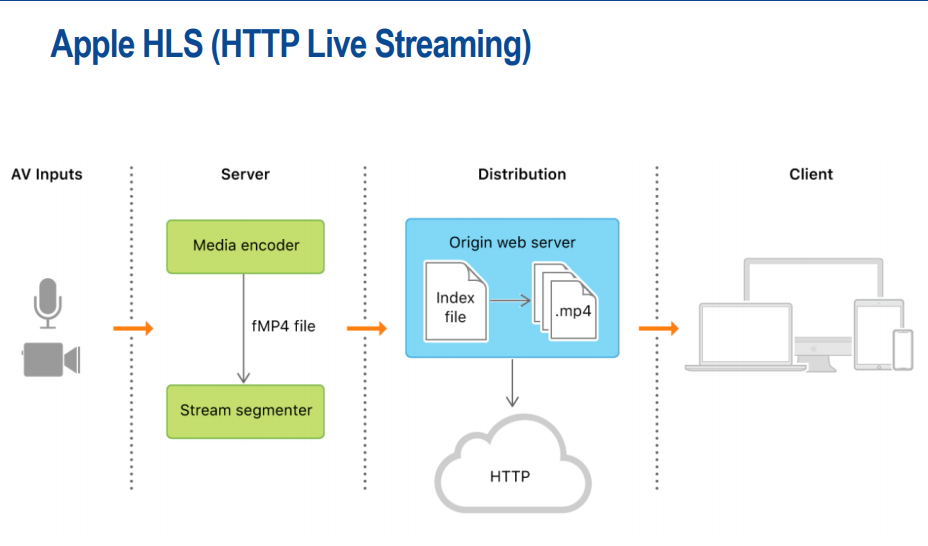
\includegraphics[width=0.85\textwidth]{images/hls.PNG}
\end{figure}

\subsubsection{HLS playlist}
Obsahuje segmenty (chunky), Je přenášen pomocí http(s) \newline
První řádek identifikuje formát, Další řádek definuje délku každého segmentu, Dále následuje popis segmentů\newline
Existence Master Playlistu -- Obsahuje různé varianty stejného obsahu (různé kódování, formát, přenosová
rychlost apod.)

\subsubsection{HLS segmenty}
Jsou odkazovány z playlistu a mají konkrétní URL, Obsahují informace pro dekódování segmetnu, Každý následující segment musí navazovat na segment předchozí, Trvání segmentu je definováno značkou EXTINF


\subsection{RTSP -- Real-time streaming protocol}
“Síťový dálkový ovladač”, port 554, Signalizační protokol pro řízení přenosu dat (např. protokolem RTP), Podporuje multicastové vysílání, Syntaxe je přirovnatelná k HTTP 
\begin{verbatim}
    (rtsp://host[:port]/[absolutní cesta])
\end{verbatim}
\textbf{RTSP metody}: \newline
PLAY (povinný), PAUSE, RECORD, SETUP (povinný), SET\_PARAMETER, \newline 
GET\_PARAMETER, OPTIONS (povinný), REDIRECT, DESCRIBE, \newline 
TEARDOWN (povinný) \newline \newline
\textbf{Funkce}:
\begin{enumerate}
    \item Získání multimediálních dat z multimediálního serveru
    \item Pozvání multimediálního serveru do konference
    \item Přidání multimediálních dat do existující prezentace
\end{enumerate}


\newpage
\section[Popište komunikaci prostřednictvím rodiny protokolů H.323, vyjmenujte čtyři základní prvky sítě H.323, popište jejich funkce. Jaké protokoly se v rámci komunikace H.323 používají pro signalizaci hovoru, kompresi AV dat a přenos AV dat.]{Popište komunikaci prostřednictvím rodiny protokolů H.323, vyjmenujte čtyři základní prvky sítě\newline H.323, popište jejich funkce.\newline Jaké protokoly se v~rámci komunikace H.323 používají pro signalizaci hovoru, kompresi AV dat a~přenos AV dat.}
\subsection{Standard H.323} 
Rodina protokolů pro audiovizuální komunikaci, Popisuje infrastrukturu audio-visuálních služeb v paketově orientovaných sítích, které nemohou zajistit garantovanou kvalitu služeb, Zajišťuje audio-vizuální komunikaci – audio komunikace je povinná

Základní prvky:
\begin{enumerate}
    \item \textbf{Terminál (Terminal)} -- koncové zariadenie -- Hardwarové a softwarové, může jít o IP telefon nebo videokonferenční systém. Komponenty: kamera, mikrofon, displej, ovladač, reproduktory, kodek, prezentační PC
    \item \textbf{Brána (Gateway)} -- Zajišťují překlad signalizace u zařízení v různých sítích (například IP vs PSTN)
    \item \textbf{Gatekeeper (Gatekeeper)} -- Volitelná komponenta, Software pro obsluhu zóny obsluhující terminály, jednotky MCU, …, v jedné zóně může být jen jeden Gatekeeper. Zajišťuje: Překlad adres (H323 ID na IP adresy), řízení šířky pásma, řízení přístupu, řízení zóny, administraci kontaktu
    \item \textbf{Vícebodová řídící jednotka MCU (Multipoint Controller Unit)} -- Řídí spojení tří a více  účastníků v jedné konferenci, Zajišťuje přepínání, mixování a kodování jednotlivých multimediálních dat.

\end{enumerate}
\textbf{Kontroler} –- řídí spojení tří a více uživatelů, poskytuje prostředky na dohodnutí způsobu komunikace s terminály \newline
\textbf{Procesor} –- provádí mixování (více streamů videa do jednoho) a přepínání (určení videa, které bude přenášeno
k uživateli)
\newline \newline
Standard H.323 zastřešuje
\begin{enumerate}
    \item \textbf{Signalizační protokoly}: H.225.0 – hovorová signalizace, H.245 – dohodnutí kodeků pro kompresi, H.225.0 RAS (Registration, Admission, Status)
    \item\textbf{ Protokoly pro přenos médií}: RTP/RTCP
    \item \textbf{Protokoly pro kompresi audio/video dat}: H.225.0 – Zajišťuje inicializaci a řízení relace, H.225.0 RAS – slouží pro vyhledání gatekeeperu pomcí multicastových skupin, H.245.0 – Slouží k dohodnutí kodeků
\end{enumerate}

\newpage
\section[Popište komunikaci prostřednictvím protokolu SIP, žádosti a odpovědi definované v doporučení RFC3261, prvky sítě SIP a základní schéma spojení bod-bod, bod-proxy server-bod.]{Popište komunikaci prostřednictvím protokolu SIP, žádosti a odpovědi definované v doporučení\newline RFC3261, prvky sítě SIP a základní schéma spojení bod-bod, bod-proxy server-bod.}
\subsection{SIP (Session Inititation Protocol)}
Textově orientovaný signalizační protokol, Zajišťuje inicializaci, modifikaci a ukončení spojení, Uplatnění – IP telefonie, konference, Instant Messaging. využívá nejčastěji UDP port 5060, ale může využít i TCP


SIP slouží pro sestavení relace mezi dvěma entitami (UA)

Síťové prvky SIP:
\subsubsection{User Agent}
\begin{enumerate}
    \item User agent (UA) -- klient nebo server (telefon, brána).
    \item User Agent Client (UAC) -- logická funkce, která generuje žádosti SIP a přijímá odpovědi SIP; telefon SIP inicializující hovor nebo SIP Proxy přeposílající žádosti k jinému UAC
    \item User Agent Server (UAS) -- logická funkce, která přijímá žádosti SIP a posílá odpovědi SIP
\end{enumerate}
\begin{figure} [h]
     \centering
     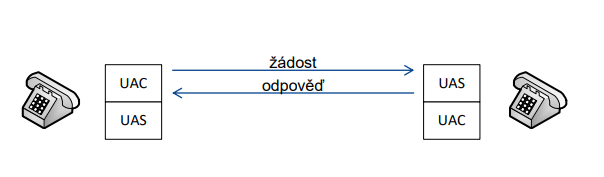
\includegraphics[width=0.85\textwidth]{images/bod-bod.PNG}
\end{figure}
\subsubsection{PROXY server}
Proxy server je mezilehlá entita, která je v sítích SIP zodpovědná za
přeposílání žádostí nebo odpovědí. Primární funkcí PROXY serveru v SIP
sítích je tedy směrování. Mimo to může také zajišťovat autentizaci a
autorizaci uživatelů.
\begin{figure} [h]
     \centering
     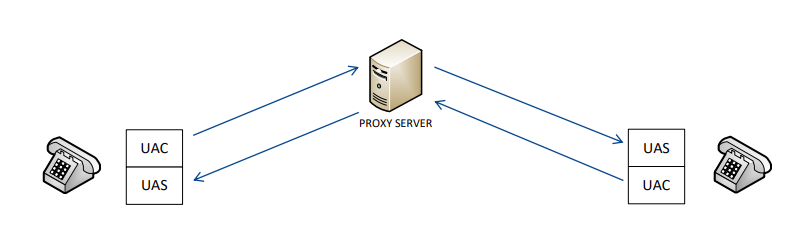
\includegraphics[width=0.85\textwidth]{images/bod-proxy.PNG}
\end{figure}

\subsubsection{REDIRECT server}
Redirect server je speciální typ UAS, který generuje odpovědi třídy 3xx,
které v sobě nesou adresu volaného. Jeho hlavním úkolem je tedy odeslat
zpět UAC adresu, na které se volaný nachází.
\begin{figure} [h]
     \centering
     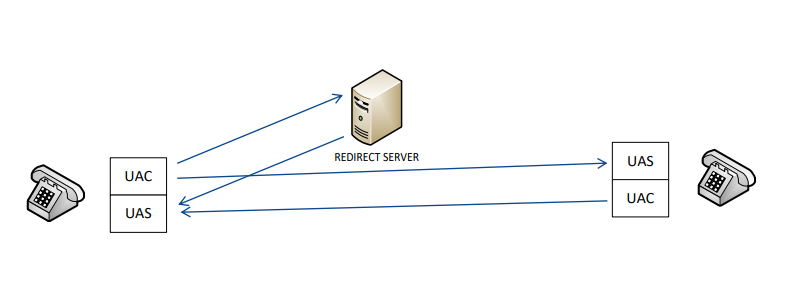
\includegraphics[width=0.85\textwidth]{images/redirect.PNG}
\end{figure}

\subsubsection{REGISTRAR server}
Registrar přijímá pouze žádosti o registraci SIP REGISTER od UAC a
aktualizuje podle nich lokalizační databázi koncových UA, které jsou v rámci
domény spravovány. Registrar udržuje v databázi SIP URI (Uniform
Resource Identifier) a IP adresy. Tato databáze se nazývá Lokační služba.
\begin{figure} [h]
     \centering
     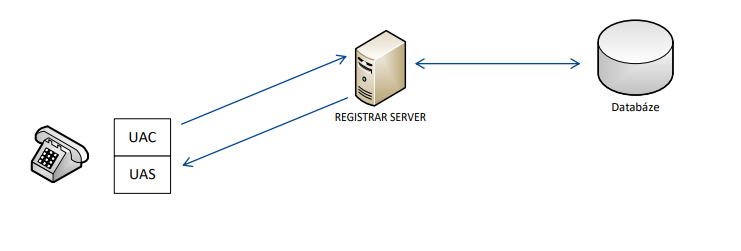
\includegraphics[width=0.85\textwidth]{images/registrar.PNG}
\end{figure}

\subsubsection{B2BUA}
generuje SIP žádosti jako UAS a SIP odpovědi jako UAC. Hovor mezi
dvěma účastníky SIP řízený B2BUA je tvořen dvěma dialogy.
\begin{figure} [h]
     \centering
     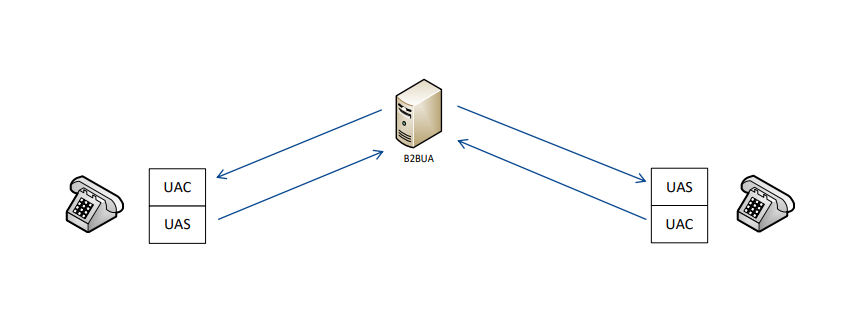
\includegraphics[width=0.85\textwidth]{images/b2bua.PNG}
\end{figure}

\subsection{Zpráva typu ŽÁDOST}
Vysílané klientem k serveru, RFC 3261 definuje 6 metod SIP
\begin{enumerate}
    \item INVITE -- indikuje, že uživatel nebo služba je pozvána k účasti v relaci. Může být také použita k modifikaci charakteristiky probíhající relace
    \item ACK -- potvrzuje, že UAC přijal finální odpověď na žádost INVITE, používá se pouze s metodou INVITE
    \item BYE -- posílá UA v případě požadavku o ukončení probíhající relace.
    \item CANCEL -- umožňuje UAC a síťovým serverům stornovat žádost, jako je například INVITE
    \item OPTIONS -- je využívána UA pro zjištění kapacity UAS
    \item REGISTER -- využívaná klientem pro registraci současné polohy odpovídající AOR SIP serveru.
\end{enumerate}

\subsection{Zpráva typu ODPOVĚĎ}
Posílá server klientovi, Indikuje stav žádosti
• Skupiny:
\begin{enumerate}
    \item 1xx – dočasné dopovědi
    \item 2xx – úspěšné zpracování žádosti
    \item 3xx – indikuje nutnost přesměrování žádosti
    \item 4xx, 5xx, 6xx – indikuje chybu při zpracování žádosti SIP
\end{enumerate}


\newpage
\section{Webinar, Webcast, Videokonference, teleprezence – popište základní rozdíly (výhody/nevýhody), využívané protokoly, standardní i proprietární).}

Společné vlastnosti:
\begin{enumerate}
    \item poskytuje komunikační prostředky pro multimediální spojení mezi dvěma a více uživateli na různých místech v reálném čase
    \item využívá síťovou strukturu TCP/IP,
    \item přenáší zvuk, obraz, text a data.
\end{enumerate}

\subsection{Webinar (webový seminář)}
Interaktivní seminář v reálném čase v síti Internet, Využívá se pro: online školení, konzultace,
prezentace

Průběh multimediální komunikace:
\begin{enumerate}
    \item přednášející prezentuje osobně obsah semináře
    \item posluchači mohou interaktivně reagovat většinou prostřednictvím textových zpráv (tzv. chat).
\end{enumerate}


\subsection{Webcast (prezentace prostřednictvím Internetu)}
Streaming (vysílání) multimediálního obsahu více příjemcům, Streaming v reálném čase (online) nebo na vyžádání, Využívá se pro: internetové rádio a televizi, školení bez interakce.

\subsection{Videokonference}
Videokonference je technologie pro vzájemnou komunikaci, Volitelně můžou být přenášena data v podobě souborů či prezentací (zaleží na užitém
systému).
Volitelně může být zařazen chat.



\subsection{Teleprezence}
Telepresence je technologie pro vzájemnou komunikaci budící dojem přímé komunikace u jednoho stolu.


\begin{figure} [h]
     \centering
     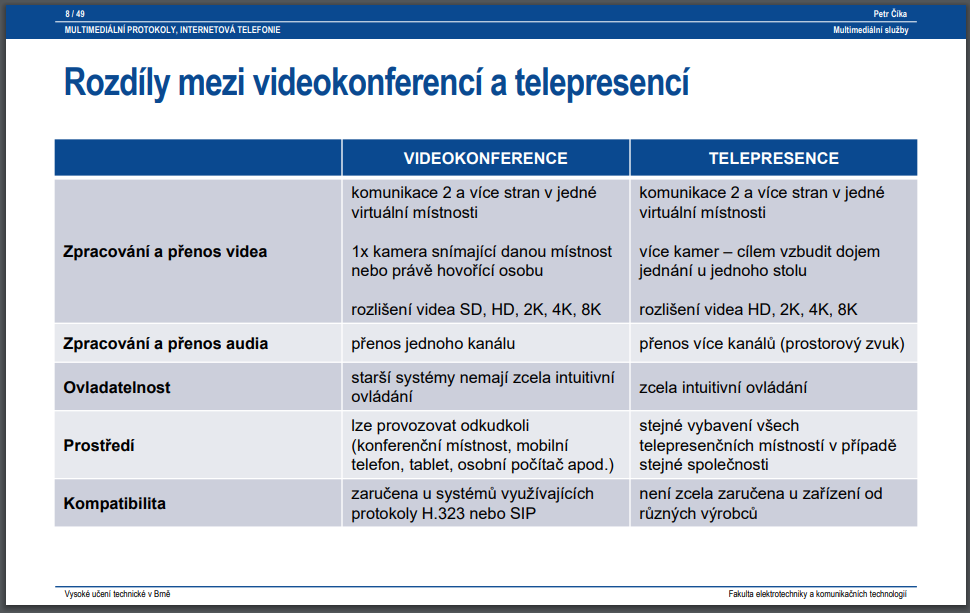
\includegraphics[width=0.85\textwidth]{images/teleVSvideo.PNG}
\end{figure}

\newpage
\textbf{Videokonference} a \textbf{teleprezence} jsou vhodné pro uspořádání plně interaktivní online komunikace více osob z různých lokalit v reálném čase:
\begin{enumerate}
    \item umožňují přenos zvuku, videa, textu a doplňkových dat (chat, sdílená obrazovka apod.) v reálném čase,
    \item umožňují vytvořit dvoubodové i vícebodové spojení
\end{enumerate}


\newpage
\section{Komprese statických obrazových dat dle standardů JPEG - základní schéma, popis jednotlivých bloků - jejich funkce.}
\subsection{JPEG -- Joint Picture Expert Group}
první mezinárodní standard pro kompresi barevných, šedotónových a černo-bílých
digitálních statických obrazů, *.jpg \newline
Podporuje ztrátovou (založenou na diskrétní kosinové transformaci (DCT) i bezeztrátovou
(založenou prediktivním kódování) kompresi

Komprese není závislá na:
\begin{enumerate}
    \item Prostorovém rozlišení obrazu
    \item Poměru stran obrazu
    \item Barevném modelu
\end{enumerate}

Celkem 4 módy kódování
\begin{enumerate}
    \item základní mód – ztrátové kódování (komp. poměr ~1:20), využívá DCT, Huffmanovo kódování
    \item rozšířený mód – ztrátové kódování , progresivní kódování, DC všech bloků, 1. AC všech bloků, atd.
    \item bezeztrátové kódování - , prediktivní kódování ,nevyužívá DCT
    \item hierarchické kódování – několik prostorových rozlišení
\end{enumerate}

\begin{figure} [h]
     \centering
     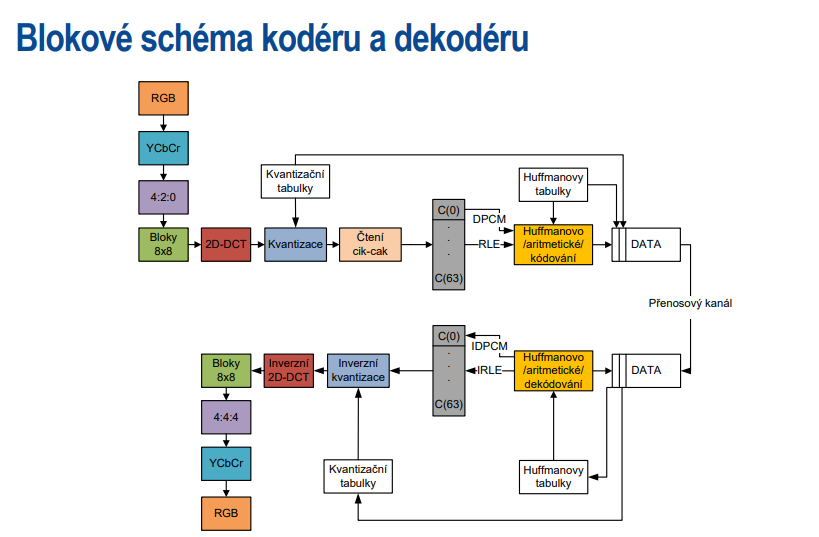
\includegraphics[width=0.9\textwidth]{images/jpeg.PNG}
\end{figure}

Blokové schéma kodéru a dekod. (obr)
\begin{enumerate}
    \item Převedení z RGB na YCbCr
    \item Podvzorkování Cb a Cr složky (jasová složka je citlivější na oko než barevná)
    \item Rozdělení na 8x8 px bloky
    \item Provedení DCT (Diskrétní kosinová transformace) – potlačení korelačních vazeb mezi vzorky, koncentrace energie signálu do oblasti nízkých frekvencí, zanedbání vyšších frekvencí, zaokrouhlení frekvenčních kvocientů, není ztrátová
    \item Kvantizace – po DCT se energie soustředí k levému hornímu rohu (nízká frekvence), koeficienty představující vyšší frekvenci mají nízké hodnoty, při vynulování koeficientů s vyššími frekvencemi dochází pouze k nepatrné ztrátě kvality - zavedení malé chyby do nízkých a velké do vysokých frekvencí, při kvantizaci dochází k zásadní ztrátě informace, kvantizační tabulky nejsou standardizované, jsou zvlášt pro jasovou a barevnou složku, kvalita výsledného obrazu je ovlivněna faktorem kvantizace
    \item Čtení zik-zak – od nejnižší po nejvyšší frekvenci, koeficienty DCT jsou čteny od nejnžší frekvence po nejvyšší
    \item Provedení Huffmanova kódování - dle Huffmanových tabulek, v datovém toku jsou uloženy Huffmanovy i kvantizační tabulky
\end{enumerate}


\newpage
\section{Komprese pohyblivých obrazových dat dle standardů MPEG - základní schéma, popis jednotlivých bloků - jejich funkce, oblast použití kodeků.}

Vývoj standardů MPEG
\begin{itemize}
    \item \textbf{M-JPEG (Motion JPEG)} -- aplikace kódování JPEG na jednotlivé snímky videa
    \item \textbf{MPEG (Motion Picture Expert Group)} -- kódování videa a přidruženého audia, možnost kódování v reálném čase, Služby na vyžádání - On-demand (VoD), pomalá komprese a rychlá dekomprese
\end{itemize}

\subsection{MPEG}
Umožňují ztrátovou kompresi videosekvence, Komprese pracuje jak s časovou, tak i s prostorovou redundancí \newline
Je multimediální standard specifikující kódování obrazu a zvuku, standard na kompresi videa

\subsubsection{MPEG-1}
\textbf{navržen pro ukládání videa na CD}, formát vzorkování 4:2:0, 25 snímků/s, bitová rychlost 1-1,4 Mb/s

\textbf{Požadavky MPEG videa}: možnost zastavení obrazu, libovolný přístup ke snímkům obrazu v určitém čase (převíjení
vpřed a vzad s přesností 0.5s), schopnost řehrávání vpřed i vzad s vyšší rychlostí než je normální rychlost videa,
synchronizace audio a video stopy při přehrávání, práce v reálném čase

\textbf{Postup kódování}:
\begin{enumerate}
    \item \textbf{Přeuspořádání snímků} -- Přeskládání GOP – postup kódování je rozdílný od postupu přehrávání
    \item \textbf{Kódování 1. snímku v GOP} -- Snímek je transformován a kvantizován jako JPEG
\item Následně je kódován pomocí VLC (Variable length coding) a uložen do bufferu, před kódováním je zároveň zpětně
transformován a kvantizován a uložen do snímkové paměti
\item \textbf{Následující snímek (P)} jde společně se snímkem ve snímkové paměti do bloku odhadu pohybu
\item \textbf{Referenční snímek} je dle vektorů pohybů přeskládán, aby se co nejvíce podobal aktuálnímu snímku (P)
\item Od aktuálního snímku je odečten přeskládaný referenční snímek a rozdíl je trasformován, kvantizován a kódován a
následně spolu s vektory pohybu uložen do bufferu
\item \textbf{třetí snímek (B)} postupuje obdobně, přeskládává následující i předešlý snímek, predikce se vybírá s nejmenším rozdílovým blokem, neukládá se do snímkové paměti
\item při dekódování odpadá část odhadu pohybu
\end{enumerate}

\begin{figure} [h]
     \centering
     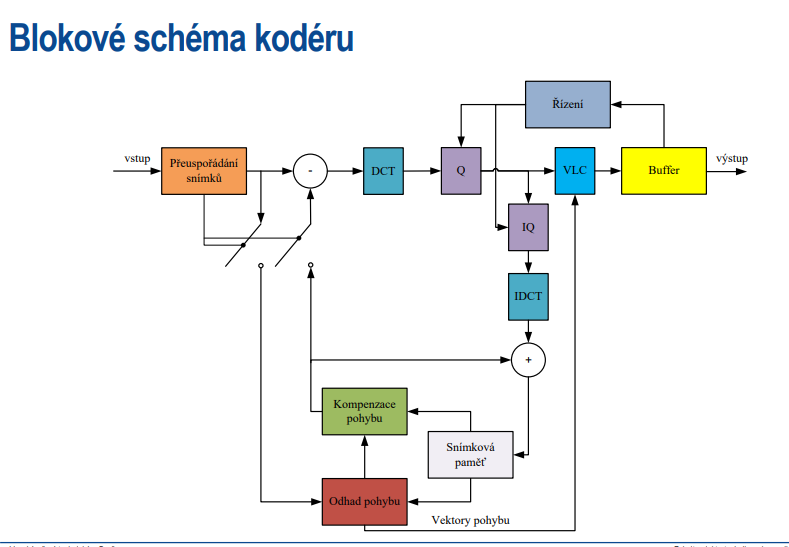
\includegraphics[width=0.9\textwidth]{images/kodovanie-mpeg.PNG}
\end{figure}

\newpage
Hierarchie:
\begin{itemize}
    \item \textbf{Sekvence} – celá videosekvence (celý film)
 \item Skupina snímků (GOP – Group of pictures) – série jednoho nebo více snímků, videosekvence se skládá ze série GOP
jdoucích po sobě, každá GOP začíná snímkem I, délka GOP je dána vzdáleností dvou I snímků, pořadí snímání GOP
se liší od pořadí kódování,
 \item \textbf{Snímek}:
 \begin{itemize}
     \item Snímek I – referenční snímek pro další snímky, kódován principem jako JPEG (první snímek GOP), jsou v něm
všechny obrazové informace,
\item Snímek P – referenční snímek, prediktivně kódován z předchozích referenčního, obsahuje pouze rozdíly oproti
předchozímu snímku, jsou o hodně menší než I snímky
\item Snímek B – není referenční pro další snímky, prediktivně kódován z předchozího i následujícího
\item Snímek D – není referenční, kódují se jako JPEG, ale pouze DC složky
\item Při kódování se standardně používá YCbCr model
 \end{itemize}
 \item \textbf{Slice} – část snímku, minimálně jeden makroblok, maximálně celý snímek
 \item \textbf{Makroblok} – 16x16 pixelů, obsahuje všechny barevné složky obrazu, MPEG-1 vzorkuje makrobloky 4:2:0 YCbCr
 \begin{itemize}
     \item Skládá se z 4x 8x8 px složky Y, 1x 8x8 px složky Cr, 1x 8x8 px složky Cb
\item Kódování makrobloků je INTRA (stejné jako JPEG, rozdílné jen kvantizační tabulky) nebo INTER (kódování rozdílu
aktuálního a referenčního makrobloku, použití u P a B snímků)
 \end{itemize}
\end{itemize}

\begin{figure} [h]
     \centering
     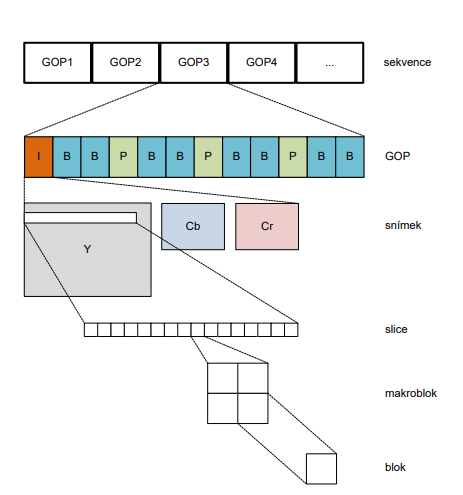
\includegraphics[width=0.7\textwidth]{images/mpeg-1.PNG}
\end{figure}

\subsubsection{MPEG-2}
Lepší kvalita obrazu, bitová rychlost 4-100 Mb/s, podpora prokládaného řádkování, kompatibilní
s MPEG1, podpora konstantní CBR tak variabilní VBR

\textbf{Využití}: DVD, BlueRay, TV, DVB-T …

\subsubsection{MPEG-4}
\textbf{Kódování objektů videa}
Efektivní komprese progresivního i prokládaného videa
Podpora:
\begin{itemize}
    \item kódování statických obrazových dat
    \item efektivního přenosu přes datové sítě 
    \item kódování animovaných objektů 
    \item kódování ve studiové kvalitě.
\end{itemize}